%\documentclass[handout]{beamer}
\documentclass{beamer}

\usepackage[english]{babel}
\usepackage[latin1]{inputenc}
\usepackage{textpos}
\usepackage{epstopdf}
\epstopdfsetup{update}
%\usepackage{pgfpages}
%\pgfpagesuselayout{resize to}[letterpaper,landscape]
%\usepackage{epstopdf}
%\epstopdfsetup{update}
\usepackage{pgfplots}
\usepackage{pgfbaseimage}
\usepackage{amsmath} 						%More mathematical
\usepackage{multirow}
%\usepackage[absolute,overlay]{textpos}
%\usepackage[tikz]{bclogo}
%\usepackage{etoolbox}
% listings for matlab code:
\usepackage{listings}
%\usepackage[autolinebreaks, useliterate]{mcode}
\lstset{backgroundcolor=\color[gray]{0.9}}

\usepackage{chemplants}
\usepackage{cancel}
\usepackage{graphicx}
\usetikzlibrary{math}
\usepackage{wasysym}
\usepackage{marvosym}

\usepackage{animate}

\usetikzlibrary{shapes.arrows}
\tikzset{My Arrow Style/.style={single arrow, draw=green!40!gray, very thick, fill=green!20!gray!10, anchor=base, align=center,text width=2cm,text=green!40!gray,rotate=-90,minimum width=0.5cm, inner sep=1mm, minimum height=0.5cm}}
\newcommand{\MyArrow}[2][]{\tikz[baseline] \node [My Arrow Style,#1] {#2};}

%-------------------------------------------------
% FOOTER
%
% Choose your footer style, by commenting other options:
%
%% - Clean: no footer, except of page number
\mode<presentation>{\usetheme{presentationTemplateBiomathFClean}}
%%  - Info: a fixed footer with basic presenter information
%\mode<presentation>{\usetheme{presentationTemplateBiomathFInfo}}
%%  - Section: Provide the sections and current section in the footer 
%\mode<presentation>{\usetheme{presentationTemplateBiomathFSection}}
%-------------------------------------------------


%voor de hand-outs
%\usepackage{pgfpages}
%\pgfpagesuselayout{2 on 1}[a4paper,border shrink=5mm]

\title{\LARGE Modelling and Simulation \normalsize of Biosystems}
\title{Modelling and Simulation of Biosystems}
\author[Daniel Illana]{Daniel Illana Gonz\'alez} %(daniel.illanagonzalez@ugent.be)}
\subtitle{Practicum 2: Modelling with ODEs}
\date{Academic year 2024-2025}


\newcommand{\mtx}[2]
  {\left[\begin{array}{#1}#2\end{array}\right]}
\newcommand{\eqset}[1]
  {\left\{\begin{array}{rcl}#1\end{array}\right.}
\newcommand{\rbar}[2]
  {\left.#1\right|_{#2}}
\newcommand{\atwp}[1]
  {\rbar{#1}{\overline{X},\overline{U}}}

\usepackage{mdframed}

\newenvironment{opgave}[2][]{%
	\mdfsetup{%
		frametitle={%
			\tikz[baseline=(current bounding box.east),outer sep=0pt]
			\node[anchor=east,rectangle,fill=gray!40]
			{\strut #1};}%
	}
	\mdfsetup{%
		innertopmargin=10pt,linecolor=white!30,%
		linewidth=0pt,topline=true,%
		frametitleaboveskip=\dimexpr-\ht\strutbox\relax%
	}
	
	\begin{mdframed}[]\relax}{%
\end{mdframed}}



% Table of contents at the beginning of each section
%\AtBeginSection[]
%{
%  \begin{frame}
%    \frametitle{Outline}
%    \tableofcontents[currentsection]
%  \end{frame}
%}

% Title page customisation
\titlegraphic{}

\begin{document}

\frame[plain]{\titlepage}


\frame{
\frametitle{Today}
\Large
\begin{itemize}
	\item Short introduction %\bigskip % \vfill
	\begin{itemize}
	\item Stochastic Differential Equations (SDE)
	\item Discrete Jump Equations (DJE) \bigskip
	\end{itemize}
	\item Example exercises
	\begin{itemize}
		\large
		\item Solving SDE problems with Catalyst 
		\item Solving DJE problems with Catalyst \bigskip
	\end{itemize}
	\item Exercises to do %\bigskip
	\begin{enumerate}
		\large
		\item Fermenter - Second order kinetics (SDE)
		\item Aging and saturated repair (SDE)
		\item Foxes and rabbits (DJE)
		\item A simple bike share system (DJE)
	\end{enumerate}
\end{itemize}
}

\frame{
\frametitle{Stochastic differential equations}
\large
ODEs
\begin{itemize}
\item model dynamics of \textbf{deterministic} system
\end{itemize}

SDEs
\begin{itemize}
\item model dynamics of a system with a \textbf{noisy component}
\end{itemize}
\vfill
SDEs can generate trends with \textbf{random fluctuations}, e.g., in:
\begin{itemize}
\item stock markets
\item population of animals or humans
\item (bio)chemical processes
\end{itemize}
\vfill
Suitable for temperature, pressure, price, very large number of species.
}



\frame{
\frametitle{Stochastic differential equations}
\Large

\begin{figure}
	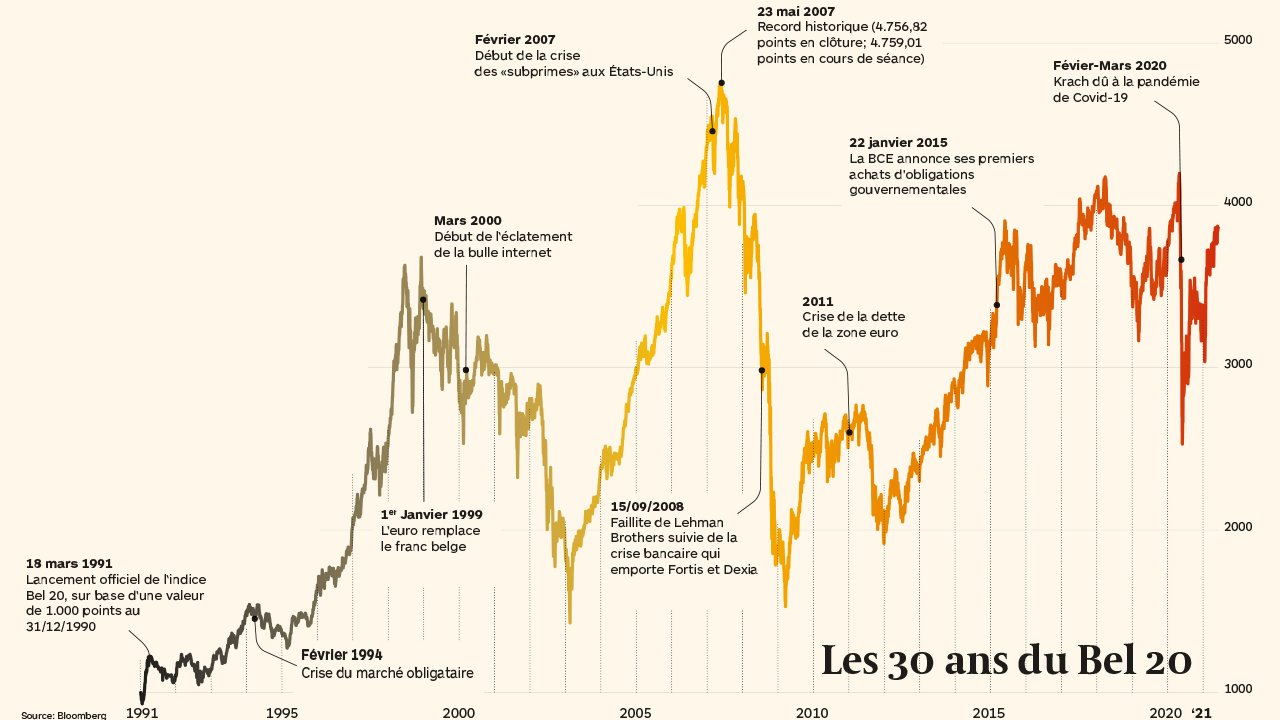
\includegraphics[width=0.8\textwidth]{figs/bel20.jpeg}
\end{figure}

}


\frame{
\frametitle{Stochastic differential equations}
\Large
In many natural systems, the noisiness originates from \textbf{Brownian motion}:

\begin{figure}
	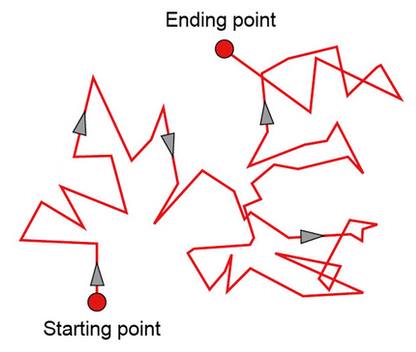
\includegraphics[width=0.5\textwidth]{figs/single_brownian_motion.png}
\end{figure}

Motion is the result of random collisions with surrounding particles.

}


\frame{
\frametitle{Stochastic differential equations}
\large
Brownian motion can be modelled by a \textbf{Wiener process}.\\
{\small A stochastic process representing a stochastic variable $W(t)$ through time:}
$$
W(t + \tau) - W(t) \sim N(0, \sqrt{\tau})
$$

\begin{figure}
	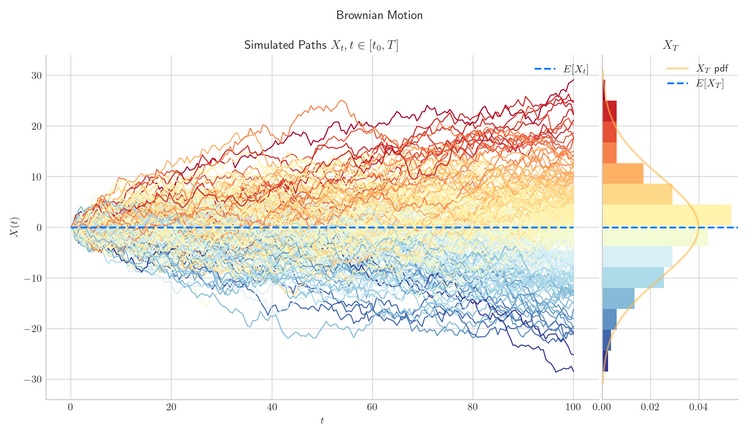
\includegraphics[width=0.6\textwidth]{figs/brownian_motions_graph.png}
\end{figure}

Generates continuous functions and $W(t)$ is a real value (${\rm I\!R}$).

}


\frame{
\frametitle{Stochastic differential equations}
\Large

A stochastic differential equation contains a deterministic part (ODE) and a stochastic part (Wiener process):
\vfill
$$
d Y(t) = \mu(Y(t), t)dt + \sigma(Y(t), t)dW_t
$$
\vfill
During the numerical calculation the variable $Y(t)$ is changing in small steps where
\begin{enumerate}
\item every step we add $\mu(Y(t), t)dt$, and then 
\item a bit of noise $dW_t$ proportional to $\sigma(Y(t), t)$
\end{enumerate}


}


\frame{
\frametitle{Discrete Jump Equations}
\Large
Many phenomena involve discrete variables, e.g.:
\begin{itemize}
\item small population of animals
\item reactions involving a limited number of species
\item traffic monitoring
\item standing in a queues
\end{itemize}

Variables are represented by natural numbers (${\rm I\!N}$).

}


\frame{
\frametitle{Discrete Jump Equations}
\Large
\begin{figure}
	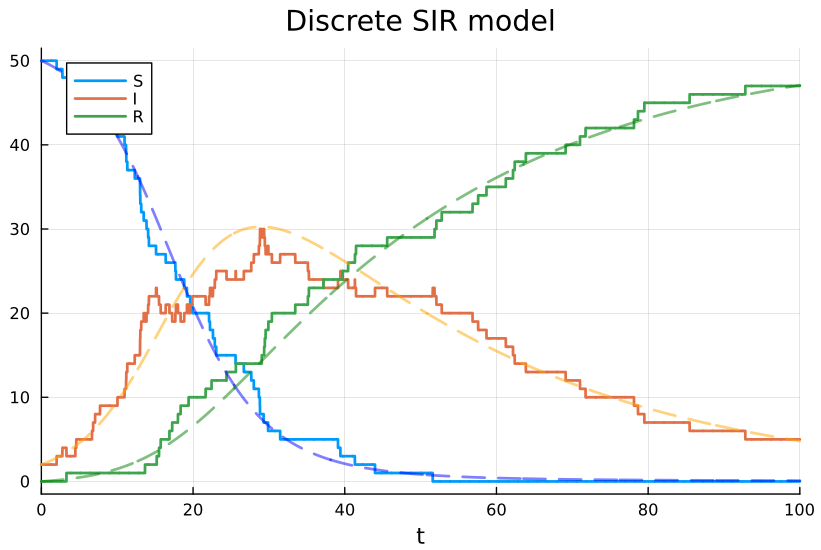
\includegraphics[width=0.8\textwidth]{figs/discrete_jump_SIR.png}
\end{figure}
}


\frame{
\frametitle{Discrete Jump Equations}
\large
\textbf{The Gillespie algorithme}
\begin{itemize}
\item The Gillespie algorithm is a way to simulate the \textit{random}, \textit{discrete events} in a system that evolves through jumps (or reactions).
\item It is widely used in chemical kinetics and population dynamics when modeling systems where changes happen at random times rather than continuously.
\item Since the process is stochastic (random), the time to the next event is not fixed but follows an \textbf{exponential distribution}.
\item Each reaction has a certain likelihood of occurring, depending on its rate which also depend on the number of reactants).
\end{itemize}

}


\frame{
  \frametitle{Goals of this practicum}
  \Large
  \color{beamerstructure}
  {\begin{enumerate}
	\item Simulating systems as SDE-problems
	\vfill %\pause
	\item Creating an ensemble problem\\
	\vfill %\pause
	\item Simulating systems as discrete jump problems
	\vfill %\pause
	\item Plotting distributions/histograms from simulations
  \end{enumerate}
  }
}


\frame{
\frametitle{Pluto notebooks}
\large

Download the exercise notebooks for today. \vfill

\begin{itemize}
\item For this practicum, go to the Ufora submodule\\ \textbf{P2: ODEs 2 $>$ files} \vfill
\item Download the Pluto notebooks and put them into your dedicated \texttt{modsim\_practica/P2\_ODE2} folder. \vfill
\item Go to your dedicated folder (cf. \texttt{modsim\_practica}) with a \textit{File Explorer}, then in this location either \vfill
\begin{itemize}
\item right click on your mouse and choose \texttt{Open in Terminal} (or something alike), or
\item write the command \texttt{cmd} in the address bar and click [\textit{Enter}].
\end{itemize} \vfill
\item Execute \texttt{julia launch\_pluto.jl} \vfill
\item Now you will be able to open and run the Pluto notebook of you choice. \vfill
\end{itemize}
}


\frame{
\frametitle{Practicum 2: ODEs 2}
\large
The following notebooks are the subjects for today:\vspace*{2mm}
\begin{itemize}
\item \texttt{sde\_model\_catalyst\_intro.jl} (introduction) \vspace*{2mm}
\item \texttt{sde\_model\_fermenter\_secondorder.jl}
\item \texttt{sde\_model\_aging.jl} \vspace*{2mm}
\item \texttt{ssa\_model\_catalyst\_intro.jl} (introduction) \vspace*{2mm}
\item \texttt{ssa\_model\_foxes\_rabbits}
\item \texttt{ssa\_model\_bike\_sharing.jl}
\end{itemize}
}



\frame{
\frametitle{SDEs problems}
\large
We will use the infection model to illustrate the following:
\begin{itemize}
\item Implementation of the system as a \textit{reaction network} object including a noise scaling parameter
\item Simulation of the system as an SDE-problem
\item Simulating the system as an ensemble problem
\item Introducing a discrete callback function
\item Analysing the results from an ensemble problem
\end{itemize}
}


\frame{
\frametitle{SDEs problems}
\Large

Notebook: \texttt{sde\_model\_catalyst\_intro.jl}

The infection model:

\begin{figure}
	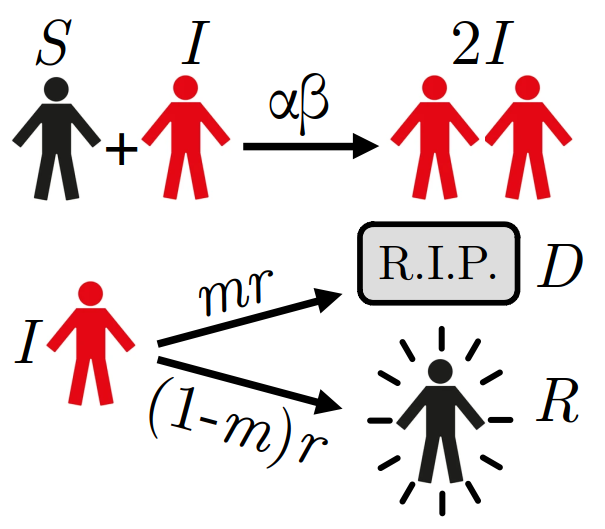
\includegraphics[width=0.6\textwidth]{figs/infection_model.png}
\end{figure}
}

\frame{
\frametitle{Exercise 1}
\Large

\textbf{Fermenter}\\
Notebook: \texttt{ode\_model\_fermenter\_secondorder.jl}

\begin{figure}
	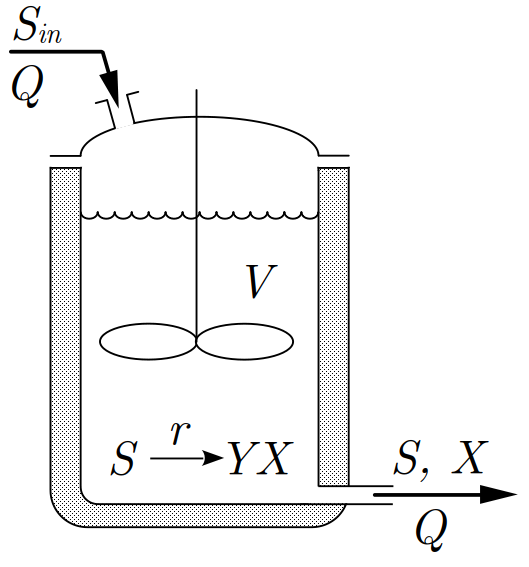
\includegraphics[width=0.5\textwidth]{figs/fermenter_model.png}
\end{figure}
}



\frame{
\frametitle{Exercise 2}
\Large
\textbf{Aging and saturated repair}\\
Notebook: \texttt{sde\_model\_aging.jl}
\vfill
{\small
$\bullet$ More senescent cells with age\\
$\bullet$ Senescent cells are being cleaned up by NK-cells\\
$\bullet$ Remaining senescent cells cause inflammation\\
}

\begin{figure}
	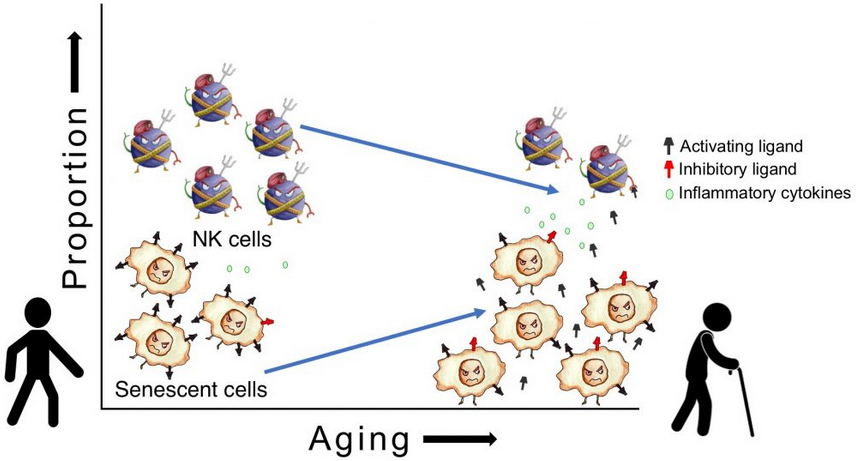
\includegraphics[width=0.7\textwidth]{figs/nk_cells_senescent_cells.png}
\end{figure}
}


\frame{
\frametitle{Exercise 2}
\Large
\textbf{Aging and saturated repair}\\
\vfill
$X$ = number of senescent cells in a human body
\vfill
Our simple model has two features:
\begin{enumerate}
\item production of damage that rises linearly with age
\item the saturating removal of damage
\end{enumerate}

$$
\cfrac{dX}{dt} = \mu t - \beta \cfrac{X}{X + \kappa}
$$
}


\frame{
\frametitle{Discrete jump problems}
\Large

Notebook: \texttt{ssa\_model\_catalyst\_intro.jl}

The infection model:

\begin{figure}
	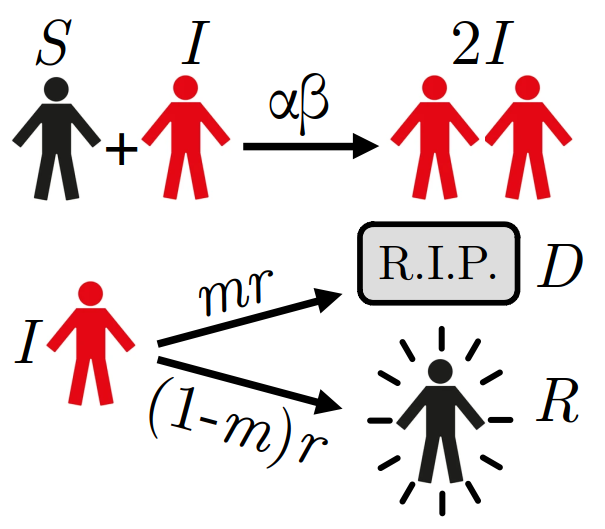
\includegraphics[width=0.6\textwidth]{figs/infection_model.png}
\end{figure}
}


\frame{
\frametitle{Exercise 3}
\Large
\textbf{Foxes and rabbits}\\
Notebook: \texttt{ssa\_model\_foxes\_rabbits}

\vspace*{2mm}

\begin{figure}
	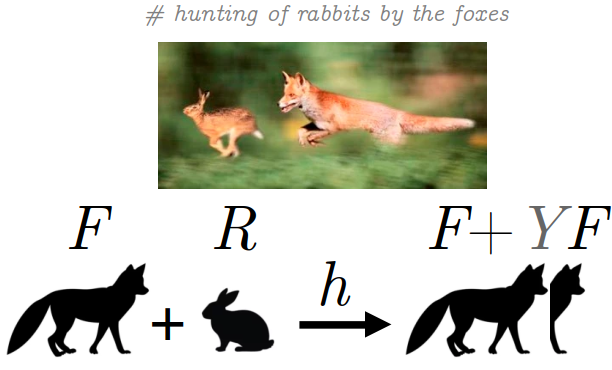
\includegraphics[width=0.7\textwidth]{figs/foxes_rabbits_model.png}
\end{figure}
}


\frame{
\frametitle{Exercise 4}
\Large
\textbf{Bike sharing}\\
Notebook: \texttt{ssa\_model\_bike\_sharing.jl}

\begin{figure}
	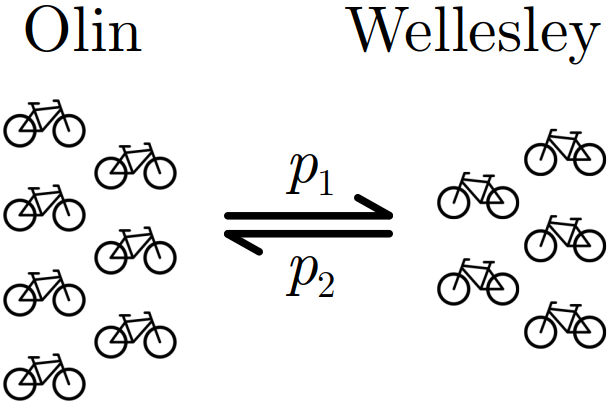
\includegraphics[width=0.8\textwidth]{figs/bike_sharing_model.png}
\end{figure}
}


\end{document}

